\documentclass[a4paper, 11pt, titlepage]{jsarticle}
\usepackage[dvipdfmx]{graphicx}
\usepackage{listings}
\usepackage{amsmath}
\usepackage{url}
\usepackage{listings,jvlisting}
\lstset{
  basicstyle={\ttfamily},
  identifierstyle={\small},
  commentstyle={\smallitshape},
  keywordstyle={\small\bfseries},
  ndkeywordstyle={\small},
  stringstyle={\small\ttfamily},
  frame={tb},
  breaklines=true,
  columns=[l]{fullflexible},
  numbers=left,
  xrightmargin=0zw,
  xleftmargin=3zw,
  numberstyle={\scriptsize},
  stepnumber=1,
  numbersep=1zw,
  lineskip=-0.5ex
}

\title{知能情報実験III(データマイニング班)\\毒のある蛇かそうでないかを画像判別}
\author{215732C 佐久本元気\\215736F 西野大河\\215742A 米須悠\\215746C 新垣樹\\}
\date{提出日:2023年8月13日}
\begin{document}
\maketitle

\begin{abstract}
 本稿では、CNN(畳み込みニューラルネットワーク)を使って画像で提示された蛇の毒の有無を予測し、正解率80\%を目標とした実験の内容や結果、考察を報告する。\par
初期段階の実験結果から、正解率を高めていくためには、データセットの前処理をしっかり行い、データ画像の枚数および蛇の種類の多様性を増やすことが必要だと仮説を立てた。また、学習モデルについてはより汎用性の高い事前学習されているVGG16をファインチューニングして利用することで正解率向上を目指すことができると考えた。中盤以降の実験に関しては、データセットへの画像の追加および、学習モデルのファインチューニング、学習反復回数の増加を行った。最終的な結果としては正解率60\%と目標に届かなかったが、実験を重ねていく中で徐々に正解率が向上したことから、機械学習ではデータセットの充実性や適切な学習回数を選択すること、蛇の分類に適した学習モデルの作成が重要であることがわかった。
\end{abstract}

\tableofcontents

\section{テーマ「毒のある蛇かそうでないかを画像判別」とは}
本グループでは画像で提示された蛇の毒の有無を予測することを対象問題として設定した。具体的な問題解決の方法としては、機械学習における画像認識・分類の技術を活用し、主にCNN(畳み込みニューラルネットワーク)を用いて行う。CNNは、\cite{theme1}によると「CNNはいくつもの深い層を持ったニューラルネットワークであり、主に画像認識の分野で価値を生んでいるネットワーク」で、「一般物体認識と呼ばれる画像認識のタスクで価値を発揮し、優れた性能を備えるアルゴリズム」とある。また、\cite{theme2}によると、「CNNの出力層はデータを解釈し、画像の予測や分類を行う」とある。
まとめると、CNNを用いることで蛇の画像の認識を行うことができ、蛇の毒の有無を予測することが可能であると考えられる。このテーマの実験を行うことの意義は、機械学習を用いた画像認識の仕方を学び、それらを様々なものに対する予測や分類に適用することができる点にあると考える。

\section{実験目的・目標}
画像に写っている蛇の毒の有無を予測し、正しいか確認することが目的である。また、予測の正答率をできる限り高めることも目的の一つである。具体的な数値としては、正解率80\%を目標とする。

\section{使用するデータの前処理}
モデルの推定精度向上を目的としデータセットに対し3種類の前処理を実行した。各々詳細を別節にて述べる。

\subsection{データセットのクレンジング}
実験毎に画像データを一枚一枚目でチェックし、クレンジングを行った。具体的には、他の動物が写っていたり、体の一部が欠けている蛇、アルビノなどノイズになりそうな画像などを各々分担しながら消去し、実験に用いた。最終的なデータセットの枚数は各実験の実験内容の節で示す。

\subsection{データの正規化}
OpenCVで画像の前処理を行い、予測を適切に行えるようにした。具体的には、$0\sim255$の数字の集合である画像データを$0\sim1$の範囲に縮小することで、学習コストの削減を試みた。

\subsection{データ分割}
ホールドアウト法を用いて、以下のような割合でデータを分割した。\par
\begin{itemize}
\item Train :70\%
\item Val:20\%
\item Test:10\%
\end{itemize}

\section{実験1}
\subsection{実験内容}
Kaggle で取得したデータセット(classification snake species\cite{theme3})を利用して実験を行った。データセットは毒蛇14,500枚、毒なし蛇26,750枚の画像で構成されている。また、データをTrain 70\%, Val 20\%, Test 10\%で分割し用意した。本実験では画像から毒あり毒無し蛇の特徴量を抽出してもらった上で予測を行うため、畳み込みやプーリングを行うことができるCNNをアルゴリズムとして採用した。そのため、学習モデルとして人がhappyかsadを識別する学習モデル(ImageClassification\cite{theme4})を採用し、sigmoid関数を用いて毒あり蛇である(出力1)、毒蛇でない(出力0)の2値を出力するようにファインチューニングを行った。\par

\subsection{パラメータ調整}
実験1ではパラメータを以下のように設定した。\par

\begin{lstlisting}[caption=パラメータ(実験1),label=fuga]
model = Sequential()
model.add(Conv2D(16, (3,3), 1, activation='relu', input_shape=(256,256,3))) 
#first layer needs to have input
model.add(MaxPooling2D())#take maximum value from 2x2 filter,only condence 

model.add(Conv2D(32, (3,3), 1, activation='relu'))
model.add(MaxPooling2D())

model.add(Conv2D(16, (3,3), 1, activation='relu'))
model.add(MaxPooling2D())

model.add(Flatten())#make it to 1D

#fully connected layers
#256neurons
model.add(Dense(256, activation='relu'))#going to have 256 values as our output
model.add(Dense(1, activation='sigmoid'))
#single output & map to 0 or1
\end{lstlisting}

以下はsummaryの結果である。\par
{\fontsize{10pt}{9pt}\selectfont
\begin{verbatim}
Model: "sequential"
_________________________________________________________________
 Layer (type)                Output Shape              Param #   
=================================================================
 conv2d (Conv2D)             (None, 254, 254, 16)      448       
                                                                 
 max_pooling2d (MaxPooling2  (None, 127, 127, 16)      0         
 D)                                                              
                                                                 
 conv2d_1 (Conv2D)           (None, 125, 125, 32)      4640      
                                                                 
 max_pooling2d_1 (MaxPoolin  (None, 62, 62, 32)        0         
 g2D)                                                            
                                                                 
 conv2d_2 (Conv2D)           (None, 60, 60, 16)        4624      
                                                                 
 max_pooling2d_2 (MaxPoolin  (None, 30, 30, 16)        0         
 g2D)                                                            
                                                                 
 flatten (Flatten)           (None, 14400)             0         
                                                                 
 dense (Dense)               (None, 256)               3686656   
                                                                 
 dense_1 (Dense)             (None, 1)                 257       
                                                                 
=================================================================
Total params: 3696625 (14.10 MB)
Trainable params: 3696625 (14.10 MB)
Non-trainable params: 0 (0.00 Byte)
_________________________________________________________________
\end{verbatim}
}

\subsection{実験結果}
\begin{figure}[htbp]
  \begin{minipage}[b]{0.45\linewidth}
    \centering
    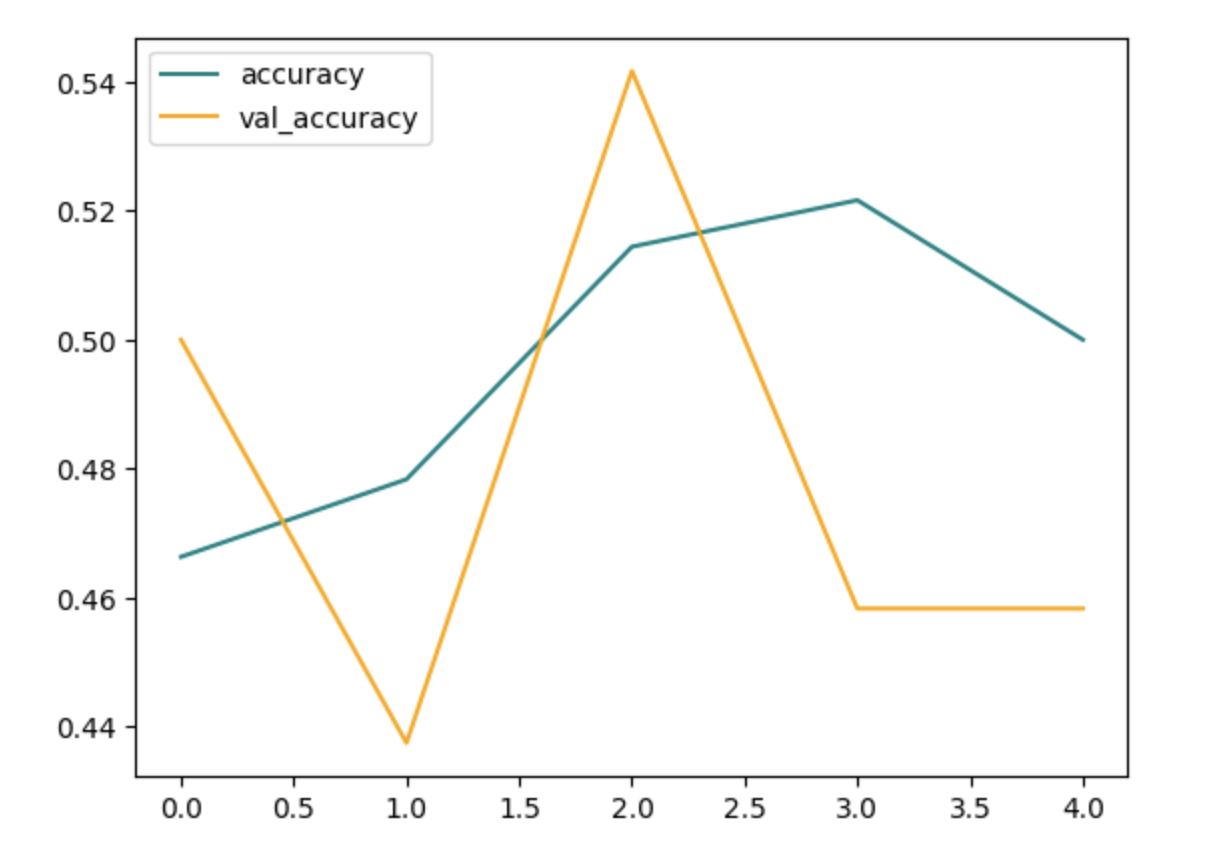
\includegraphics[keepaspectratio, scale=0.32]{ex1_acc.png}
    \caption{実験1 Accuracy}
  \end{minipage}
  \begin{minipage}[b]{0.45\linewidth}
    \centering
    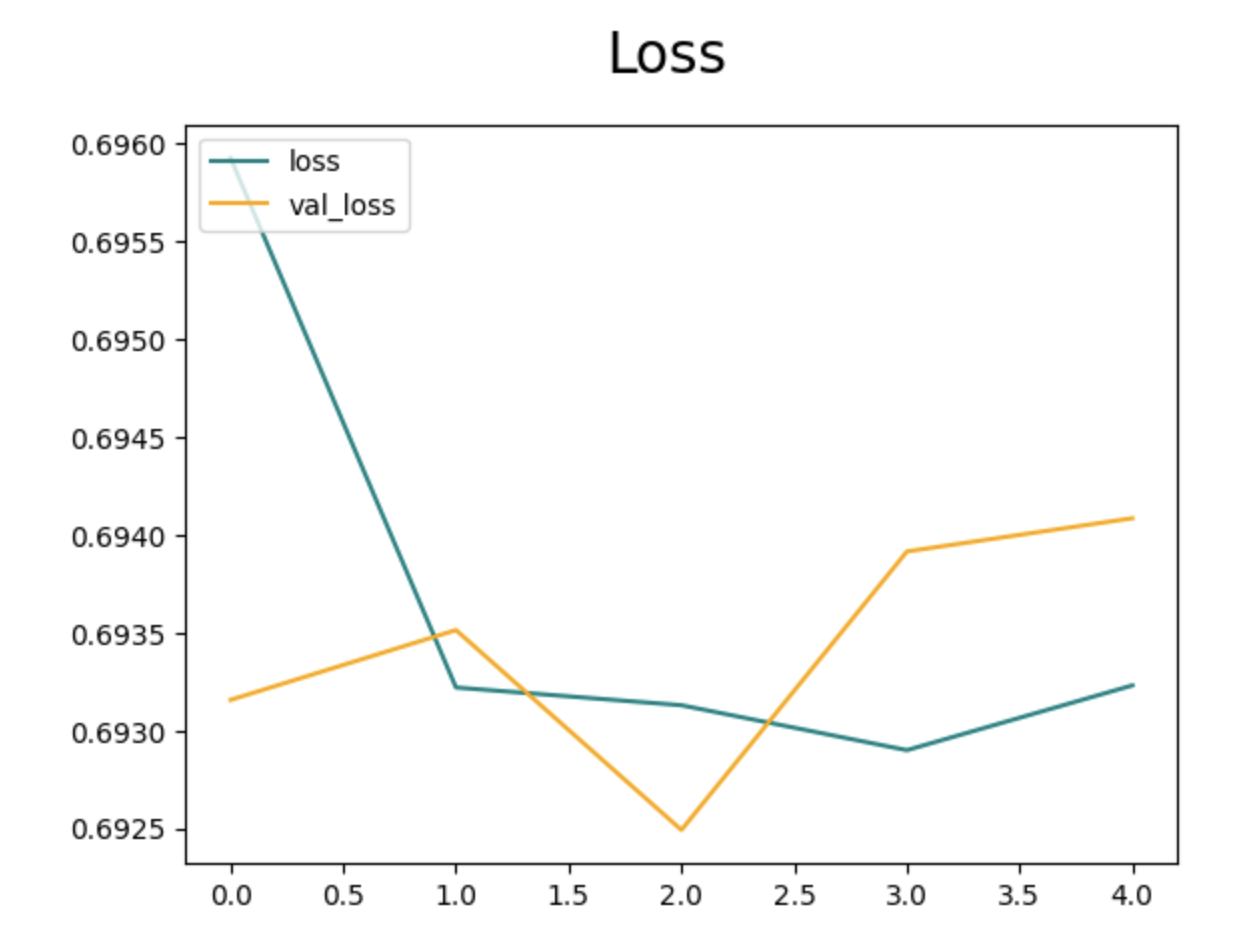
\includegraphics[keepaspectratio, scale=0.32]{ex1_loss.png}
    \caption{実験1 Loss}
  \end{minipage}
\end{figure}

\subsubsection{学習モデルの評価}
\begin{table}[htb]
\centering
  \caption{学習モデルの評価(実験1)}
  \begin{tabular}{|c|c|c|}  \hline
    適合率 & 再現率 & 正解率 \\ \hline
    0.45 & 1.00 & 0.45 \\ \hline
  \end{tabular}
\end{table}

\subsection{考察}
うまくいかなかった原因として、データセットと学習モデル両方に問題があったと考えられる。データセットは、kaggleで取得したデータセットを利用したが、体の一部が無い絶命状態の蛇や、人間の写真など投稿者のプライベート画像が大量に混入しており、信頼性のないものであった。学習モデルは、学習反復回数が5回のみで非常に少なかったことが挙げられる。また、過学習対策を行わなかったことも原因の一つとして挙げられる。他にも、蛇の画像を識別するのに、人間の表情を見分ける学習モデルを用いたことも原因として挙げられる。\par
実験1から学んだ改善点として、データセットに関しては、より適切なデータセットを探した上で、データのクレンジングを行うことが挙げられる。また、毒蛇と無毒蛇を種類ごとに調べ、データセットに追加することで、正確性を高められると考えた。学習に関しては、学習回数が足りてないように感じたため、学習反復回数を5回から20回に増やすことが挙げられた。また、VGG16のような汎用的な学習済みモデルにファインチューニングを施すことや、過学習による汎化性能の低下の対策として、NNモデルにdropout layerを追加することが挙げられた。\par

\section{実験2}
\subsection{実験内容}
学習済みモデルの作成および学習モデルの評価を行う。実験1の考察を踏まえ、新たなデータセットdataset1を作成・使用して学習する。dataset1は、無作為に選んだ毒蛇・毒なし蛇の画像(ハブやアカマタ等16種)を毒蛇・毒なし蛇それぞれ300枚、合計約600枚程度集めたデータセットである。画像収集にはGoogle Chromeの拡張機能であるImage downloader - Imageye\cite{theme6}を利用した。また、上述のデータセットとは異なる、インドの毒蛇と毒なし蛇が含まれている信頼性の高いデータセットであるindian datasetsを用いて再テストを行う。indian datasetsは毒蛇1140枚、毒なし蛇630枚の画像で構成されている。\par
モデルに関しては、実験1と同様にCNNを用いるが、すでに事前学習されているVGG16の全結合層以外のレイヤーにオリジナルでlayerを追加し、追加分レイヤーだけをファインチューニングして利用する。オリジナルで追加したlayerの特徴としてはロバストネスのためのDropout layerを用いている。\par

\subsection{パラメータ調整}
実験2ではパラメータを以下のように設定した。\par
\begin{lstlisting}[caption=パラメータ(実験2),label=fuga]
#save as txt file to view?
#create sequential neural network model. add layers with model.add.
model = Sequential()

model.add(base_model)

#additional convolution layers
model.add(Conv2D(64, kernel_size=3, padding="same", activation="relu"))
model.add(MaxPooling2D())
model.add(Dropout(0.25))

#fully connected layers
model.add(Flatten())
model.add(Dense(256, activation='relu'))
model.add(Dropout(0.5))
model.add(Dense(128, activation="relu")) 
model.add(Dense(64, activation="relu")) 
model.add(Dropout(0.5))

#use the softmax function
model.add(Dense(1, activation='sigmoid'))

\end{lstlisting}\par
以下はsummaryの結果である。\par
{\fontsize{10pt}{9pt}\selectfont
\begin{verbatim}
Model: "sequential_1"
_________________________________________________________________
 Layer (type)                Output Shape              Param #   
=================================================================
 vgg16 (Functional)          (None, 8, 8, 512)         14714688  
                                                                 
 conv2d_1 (Conv2D)           (None, 8, 8, 64)          294976    
                                                                 
 max_pooling2d_1 (MaxPoolin  (None, 4, 4, 64)          0         
 g2D)                                                            
                                                                 
 dropout_3 (Dropout)         (None, 4, 4, 64)          0         
                                                                 
 flatten_1 (Flatten)         (None, 1024)              0         
                                                                 
 dense_4 (Dense)             (None, 256)               262400    
                                                                 
 dropout_4 (Dropout)         (None, 256)               0         
                                                                 
 dense_5 (Dense)             (None, 128)               32896     
                                                                 
 dense_6 (Dense)             (None, 64)                8256      
                                                                 
 dropout_5 (Dropout)         (None, 64)                0         
                                                                 
 dense_7 (Dense)             (None, 1)                 65        
                                                                 
=================================================================
Total params: 15313281 (58.42 MB)
Trainable params: 598593 (2.28 MB)
Non-trainable params: 14714688 (56.13 MB)
_________________________________________________________________
\end{verbatim}
}\par
実験の際には、VGG16の全結合層以外のレイヤーを用い、その下にlayerを追加した。
これらの重みに関しては、VGG16モデルの重みをImageNetデータセットから事前に学習されたものに設定された状態のままにしておくため、これの重みは更新しないこととする。
オリジナルで追加したlayerにのみ重みを更新することとする。

\subsection{実験結果}
\begin{figure}[htbp]
  \begin{minipage}[b]{0.45\linewidth}
    \centering
    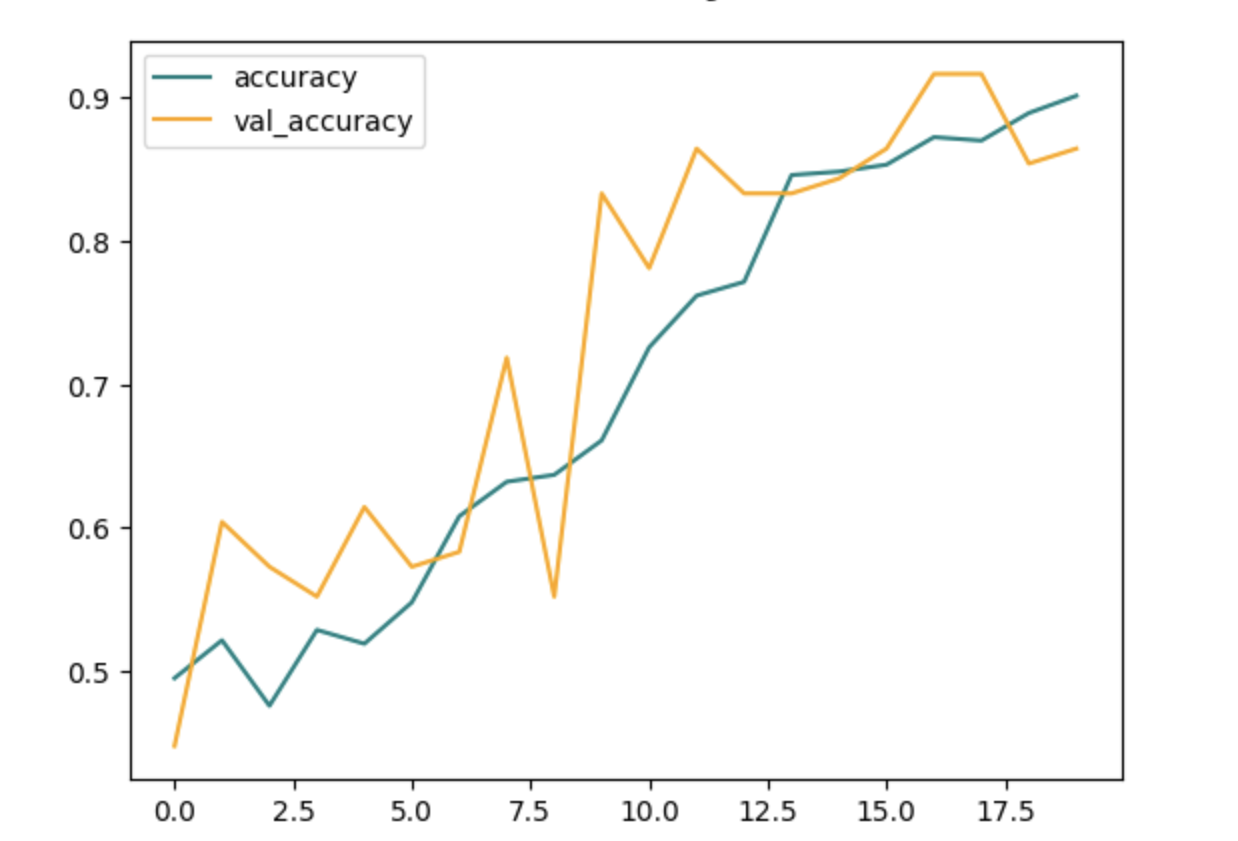
\includegraphics[keepaspectratio, scale=0.33]{ex2_acc.png}
    \caption{実験2 Accuracy}
  \end{minipage}
  \begin{minipage}[b]{0.45\linewidth}
    \centering
    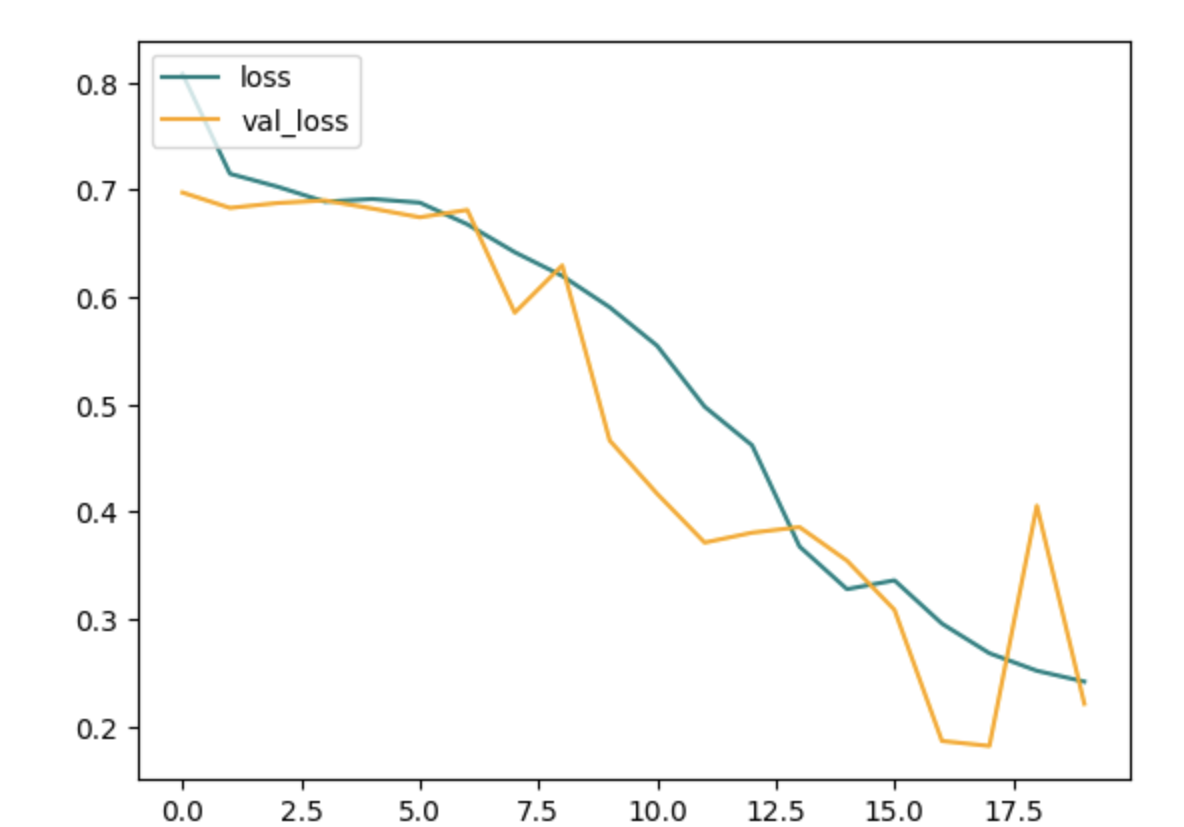
\includegraphics[keepaspectratio, scale=0.33]{ex2_loss.png}
    \caption{実験2 Loss}
  \end{minipage}
\end{figure}

\subsubsection{学習モデルの評価}
\begin{table}[htb]
\centering
  \caption{学習モデルの評価(実験2)}
  \begin{tabular}{|c|c|c|}  \hline
    適合率 & 再現率 & 正解率 \\ \hline
    0.97 & 0.76 & 0.86 \\ \hline
  \end{tabular}
\end{table}

\clearpage

\subsubsection{indian datasetsによる精査}
\begin{table}[htb]
\centering
  \caption{indian datasetsによる精査(実験2)}
  \begin{tabular}{|c|c|c|}  \hline
    適合率 & 再現率 & 正解率 \\ \hline
    0.61 & 0.39 & 0.45 \\ \hline
  \end{tabular}
\end{table}

\subsection{考察}
実験2で用いた訓練用データセットの蛇の種類は、主に日本の蛇が中心だったため、indian datasetsの特徴量と合致していなかったと考えられる。元々、毒蛇共通の特徴があると仮定して実験を行なっていたが、どちらにせよ外国の蛇のデータは必要だと考えた。\par
また、今回用いたデータセットに世界各国の毒蛇と無毒蛇の画像をそれぞれ追加することが必要だと考えた。膨大な種類の画像が必要になるため、今後の開発ではデータセットを作成する人員を増やして実験を進めていくべきだと考えられる。

\section{実験3}
\subsection{実験内容}
実験2で作成した学習済みモデルを利用し、同様に学習モデルの評価を行う。実験2の考察を踏まえ、新たなデータセットdataset2を用いて学習する。dataset2は、実験2で訓練用データセットとして用いたdataset1に世界各地の毒蛇、毒なし蛇の画像を追加したデータセットである。具体的な作成方法としては、まず地域を北アメリカ州、南アメリカ州、アフリカ州、ヨーロッパ州、アジア州(さらに東南アジア、南アジア、中央アジア、西アジアに分ける)、オセアニア州に分け、各地域ごとに毒蛇、毒なし蛇を各$2\sim5$種類選定する。その中から地域ごとの蛇の画像が合計5枚になるようにデータセットに追加した。最終的に毒蛇・毒なし蛇それぞれ約340枚、合計約680枚のデータセットとなった。画像収集には実験2同様、Image downloader - Imageyeを利用した。その後、indian datasetsを用いて精査を行う。\par

\clearpage

\subsection{実験結果}
\begin{figure}[htbp]
  \begin{minipage}[b]{0.45\linewidth}
    \centering
    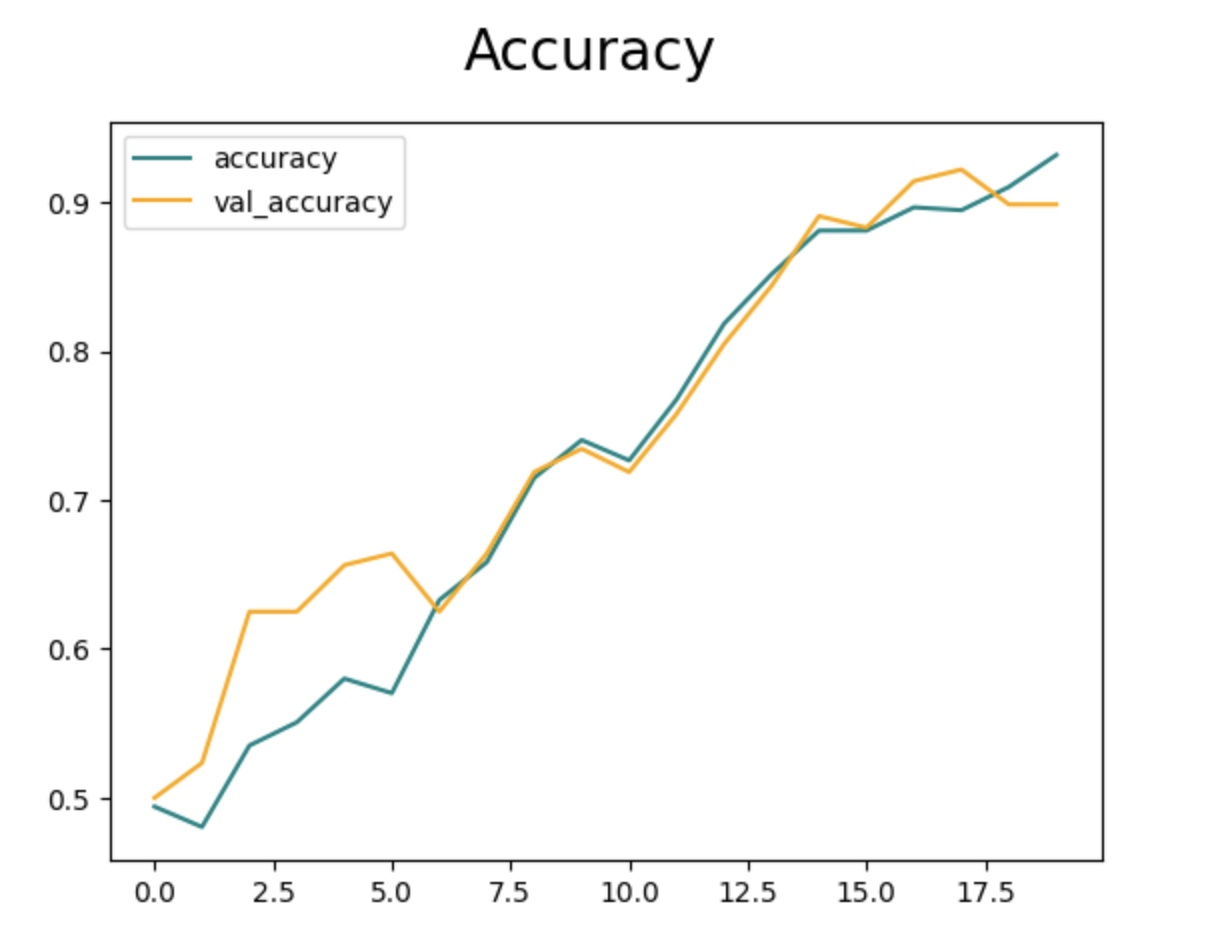
\includegraphics[keepaspectratio, scale=0.161]{ex3_acc.jpg}
    \caption{実験3 Accuracy}
  \end{minipage}
  \begin{minipage}[b]{0.45\linewidth}
    \centering
    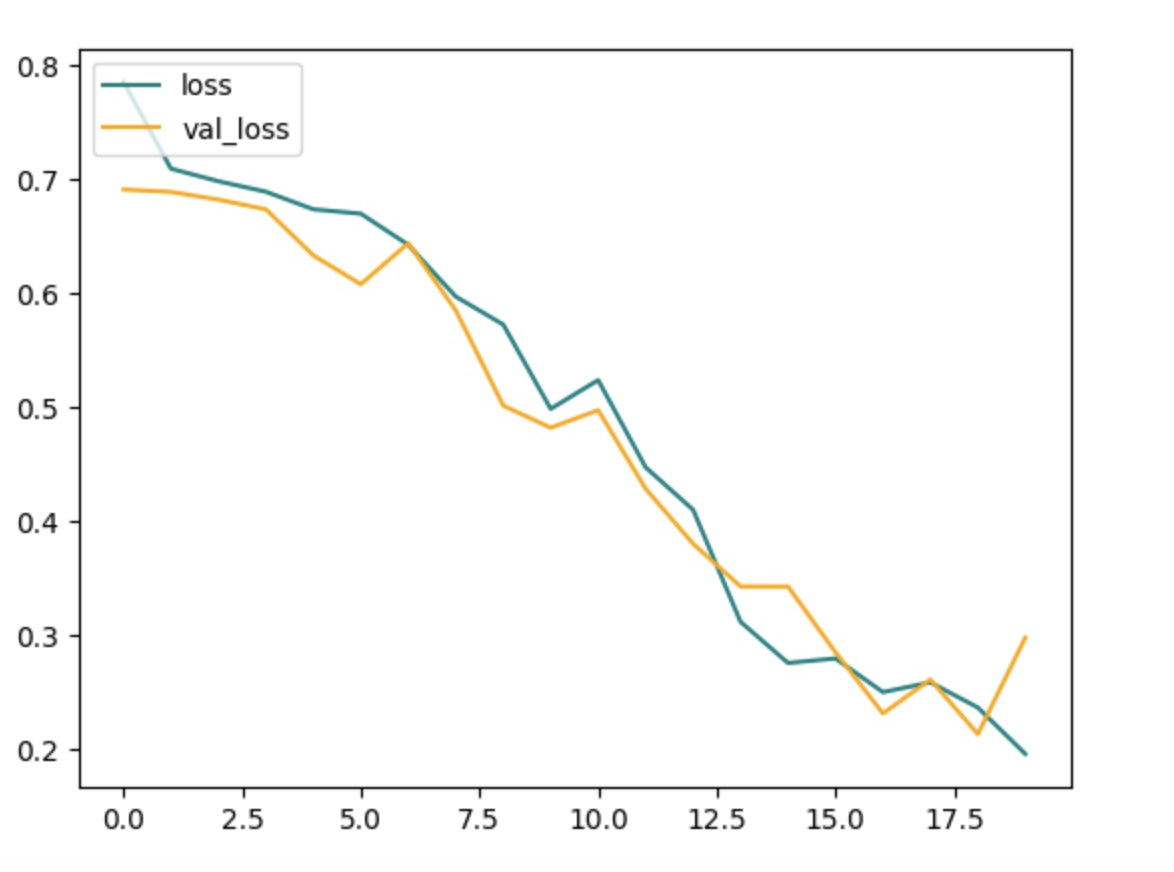
\includegraphics[keepaspectratio, scale=0.161]{ex3_loss.jpg}
    \caption{実験3 Loss}
  \end{minipage}
\end{figure}

\subsubsection{学習モデルの評価}
\begin{table}[htb]
\centering
  \caption{学習モデルの評価(実験3)}
  \begin{tabular}{|c|c|c|}  \hline
    適合率 & 再現率 & 正解率 \\ \hline
    0.97 & 0.82 & 0.91 \\ \hline
  \end{tabular}
\end{table}

\subsubsection{indian datasetsによる精査}
\begin{table}[htb]
\centering
  \caption{indian datasetsによる精査(実験3)}
  \begin{tabular}{|c|c|c|}  \hline
    適合率 & 再現率 & 正解率 \\ \hline
    0.71 & 0.53 & 0.56 \\ \hline
  \end{tabular}
\end{table}

\subsection{考察}
画像を追加したデータセットの内容は一種ごとで10倍の差があっため、外国の蛇に対する特徴量は導きにくいと予想した。一方、精査結果のスコアが向上していたため、さらにデータセットを充実させれば目標に達する可能性があると考えられる。\par
そこで、データセットに追加する分の画像を蛇一種あたり30枚ほどに増加させることで、正解率向上を目指せるのではないかと考えた。なお、追加する蛇の種類はすでに確定しており、実験2での画像追加より作業量は多くならないと見込まれるため、データセットを作成する人員を減らして進める。\par

\section{実験4}
\subsection{実験内容}
実験2で作成した学習済みモデルを利用し、同様に学習モデルの評価を行う。実験3の考察を踏まえ、新たなデータセットdataset3を用いて学習した。dataset3は、実験3で訓練用データセットとして用いたdataset2に各地域ごとの蛇の画像をさらに追加したデータセット。画像収集には実験2,3同様、Image downloader - Imageyeを利用した。その後、indian datasetsを用いて精査を行う。なお、dataset3で追加した枚数の内訳は以下の通りである。\par

\begin{table}[htb]
\centering
  \caption{データセット3に追加した枚数の内訳}
  \begin{tabular}{|c|c|c|}  \hline
    地域 & 毒あり & 毒なし \\ \hline \hline
    北アメリカ州 & 96 & 120 \\ \hline
    南アメリカ州 & 135 & 60 \\ \hline
    アフリカ州 & 143 & 80 \\ \hline
    ヨーロッパ州 & 148 & 100 \\ \hline
    東南アジア & 89 & 60 \\ \hline
    南アジア & 143 & 180 \\ \hline
    中央アジア & 54 & 30 \\ \hline
    西アジア & 61 & 90 \\ \hline
    オセアニア州 & 91 & 30 \\ \hline \hline
    合計 & 960 & 750 \\ \hline
  \end{tabular}
\end{table}

\subsection{実験結果}
\begin{figure}[htbp]
  \begin{minipage}[b]{0.45\linewidth}
    \centering
    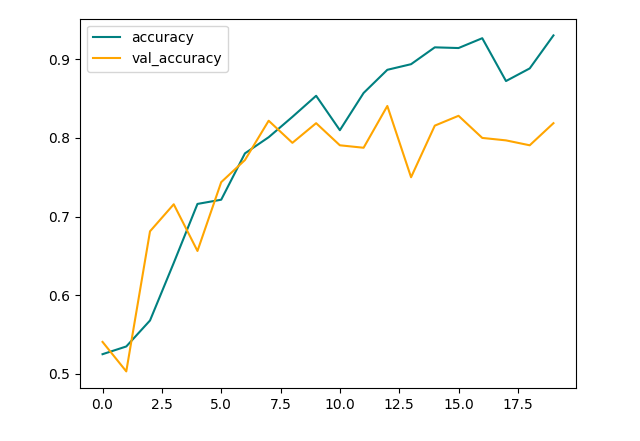
\includegraphics[keepaspectratio, scale=0.435]{ex4_acc.png}
    \caption{実験4 Accuracy}
  \end{minipage}
  \begin{minipage}[b]{0.45\linewidth}
    \centering
    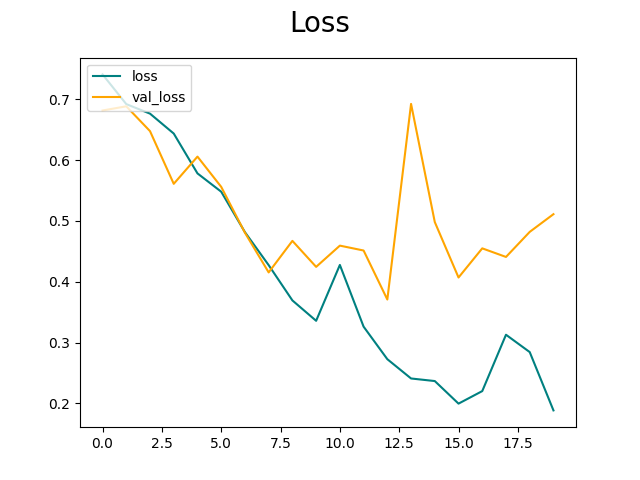
\includegraphics[keepaspectratio, scale=0.435]{ex4_loss.png}
    \caption{実験4 Loss}
  \end{minipage}
\end{figure}

\subsubsection{学習モデルの評価}
\begin{table}[htb]
\centering
  \caption{学習モデルの評価(実験4)}
  \begin{tabular}{|c|c|c|}  \hline
    適合率 & 再現率 & 正解率 \\ \hline
    0.82 & 0.94 & 0.84 \\ \hline
  \end{tabular}
\end{table}

\subsubsection{indian datasetsによる精査}
\begin{table}[htb]
\centering
  \caption{indian datasetsによる精査(実験4)}
  \begin{tabular}{|c|c|c|}  \hline
    適合率 & 再現率 & 正解率 \\ \hline
    0.70 & 0.70 & 0.61 \\ \hline
  \end{tabular}
\end{table}

\subsection{考察}
うまくいかなかった原因として、Train,Val,Testデータにそれぞれデータの偏りがあったことが挙げられる。また、データセットの画像が多すぎたことから、ノイズを完全に取り除けていなかった可能性があった。\par
改善点として、交差検証を行うことが挙げられる。本実験は、ホールドアウト法で行なっていたため、データの偏りを考慮していなかった。また、説明変数を減らして汎化性能を高めるために、正則化の実装が挙げられる\cite{theme7}。

\clearpage

\section{意図していた実験計画との違い}
行った実験の流れをガントチャートを用いて、表すと以下の通りになった。\par
\begin{figure}[htbp]
\begin{center}
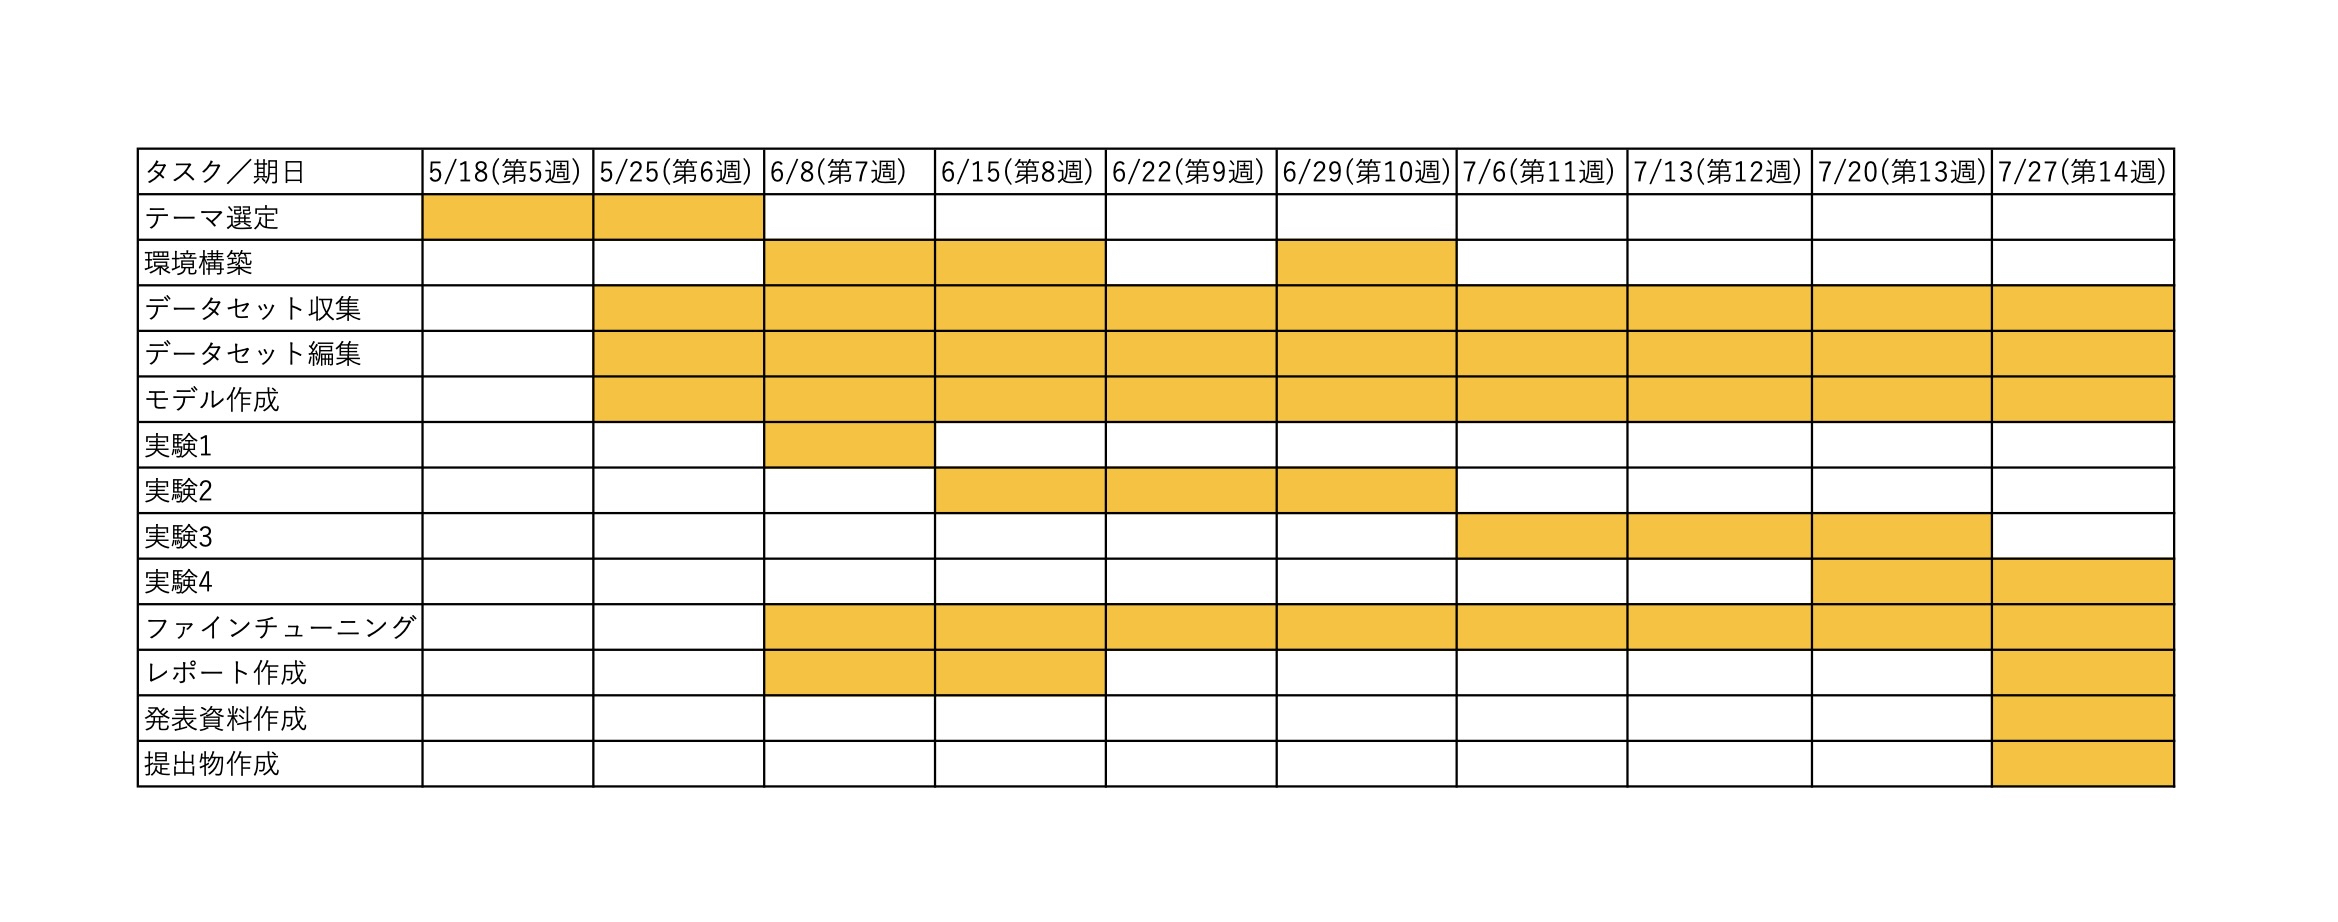
\includegraphics[width=150mm]{G2_Ganttchart.jpeg}
\caption{実験の流れ}
\end{center}
\end{figure}
想定していた以上に環境構築で躓いてしまい、本来1週で構築する予定だったが3週ほどかかってしまった。データセットに関しては、開発期間全体を通して収集・編集をおこない、正答率向上を目指した。

\section{まとめ}
今回の実験では、画像に写っている蛇の毒の有無を予測し、正しいか確認することを目的として、正解率80\%を目指して実施した。残念ながら、最終的な正解率は約60\%と目標を達成することができなかった。しかし、実験の中で気づいた点として、「データセットの充実性」についての重要性が挙げられる。データセットをテスト用のデータに対応させるために工夫するたび、正解率が上がっていったことから、機械学習におけるデータセット内容の重要性について再認識することができた。また、実験を進めていくにつれ、機械学習の手法や開発に対する取り組み方についての理解を深めることができた。他にもGitHubを利用したバージョン管理や学科サーバーを利用した実験なども行うことができ、チーム開発として良い点だったと考える。

\begin{thebibliography}{n}
	\bibitem{theme1}画像認識でよく聞く「CNN」とは?仕組みや特徴を1から解説, \url{https://aismiley.co.jp/ai_news/cnn},2023/06/14.
	\bibitem{theme2}画像認識の分野では欠かせない「CNN(畳み込みネットワーク)とは」, \url{https://www.paloaltoinsight.com/2022/12/09/cnn},2023/06/14.
	\bibitem{theme3}classification snake species, \url{https://www.kaggle.com/datasets/nikhilshingadiya/sample-0},2023/06/08
	\bibitem{theme4}ImageClassification,\url{https://github.com/nicknochnack/ImageClassification},2023/06/08
	\bibitem{theme5}Indian-Snakes-Dataset, \url{https://github.com/arjun921/Indian-Snakes-Dataset},2023/06/08
	\bibitem{theme6}Image downloader - Imageye, \url{https://chrome.google.com/webstore/detail/image-downloader-imageye/agionbommeaifngbhincahgmoflcikhm},2023/06/15
	\bibitem{theme7}NRI 野村総合研究所 用語解説 過学習\url{https://www.nri.com/jp/knowledge/glossary/lst/ka/overfitting},2023/08/03
\end{thebibliography}
\end{document}
